\section{Sensitivity to Aggregation}
\label{app:weighting}

Table~\ref{tab:weighting} contrasts equal simulation weighting with equal roommate-record weighting. The latter reproduces the mean scores in the supplied overall standings. It emphasizes configurations with many copies of a group, including the large homogeneous households that often ran short of socks. Group 4 ranks eighth under equal simulation weighting and ninth under equal roommate weighting. Neither convention changes the conclusion that its shortage control needs improvement. Since every configuration has three repetitions, equal configuration weighting after averaging seeds is identical to equal simulation weighting.

The broad conclusion also holds for each seed separately. Group 4's equally weighted mean scores were 926.44, 923.09, and 921.34 for seeds 1, 2, and 3, respectively. It ranked eighth in each case. Several other groups had overlapping ranges of seed-specific means, so their smaller overall differences should be interpreted cautiously.

\begin{table}[htbp]
\centering
\begin{tabular}{rrrrr}
\toprule
& \multicolumn{2}{c}{Equal simulation weight} & \multicolumn{2}{c}{Equal roommate weight}\\
Group & Mean daily score & Rank & Mean daily score & Rank\\
\midrule
1 & 887.33 & 1 & 3462.11 & 5\\
2 & 890.14 & 4 & 3461.12 & 4\\
3 & 889.05 & 2 & 3451.25 & 2\\
\textbf{4} & \textbf{923.63} & \textbf{8} & \textbf{3856.68} & \textbf{9}\\
6 & 893.10 & 7 & 3477.23 & 7\\
7 & 889.73 & 3 & 3447.41 & 1\\
8 & 891.03 & 6 & 3463.61 & 6\\
9 & 941.96 & 9 & 3724.65 & 8\\
10 & 890.20 & 5 & 3460.55 & 3\\
\bottomrule
\end{tabular}
\caption{Sensitivity of overall scores and ranks to the unit of aggregation.}
\label{tab:weighting}
\end{table}
\FloatBarrier

\clearpage
\section{Changes in Other Groups' Outcomes}
\label{app:externalities}

To examine Group 4's association with outcomes for its neighbors, we matched five-person rosters sharing four groups and differing only in the fifth. For each other group, we compared replacing that group with Group 4 while holding the draw size, drawer multiplier, budget, duration, and seed fixed. There were 10,080 comparisons per replaced group. Figure~\ref{fig:externalities} reports the change in the average score of the four groups retained in both rosters, so the comparison does not include the incoming player's own score.

The changes were small relative to the total scores in five-person households. Replacing Group 1 with Group 4 increased the other four groups' total embarrassment by 1.70 per roommate-day but reduced their mismatch component by 0.080. Replacing Group 2 reduced their total score by 0.159 while increasing the mismatch component by 0.067. These examples again show that matching and sock availability can move in opposite directions. Household spending also changed differently by replaced group: replacing Group 1 reduced annual spending by \$12.28 on average, whereas replacing Group 2 increased it by \$47.94.

These are comparisons within the tested roster and resource grid, not evidence that Group 4 universally helps or harms its neighbors. Matched seeds do not preserve identical random trajectories once sock choices and replacements diverge. Individual discard histories and daily drawer contents would be needed to identify the mechanisms behind the changes.

\begin{figure}[htbp]
\centering
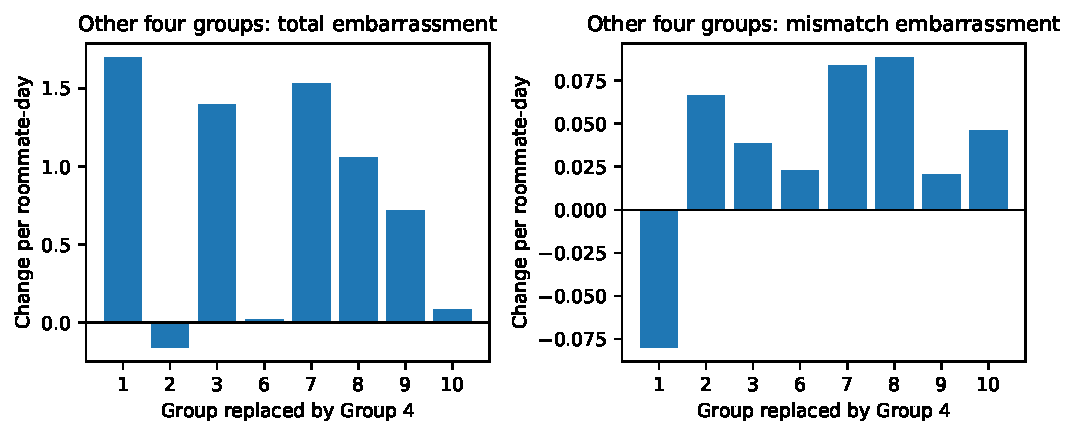
\includegraphics[width=\textwidth]{report/analysis/figures/07_externalities.pdf}
\caption{Changes for the four retained groups when the fifth roommate's strategy is replaced by Group 4. Each bar averages 10,080 matched comparisons. Positive values mean greater embarrassment for the retained groups.}
\label{fig:externalities}
\end{figure}
\FloatBarrier
